\documentclass[11pt,a4paper]{article}

\usepackage[polish]{babel}
\usepackage[utf8]{inputenc}
\usepackage{polski}
\usepackage[T1]{fontenc}
\usepackage{indentfirst}
\usepackage{wrapfig}    % for wrapping figures, tables
\usepackage{isotope}
\usepackage{hyperref}
\usepackage{amsmath}
\usepackage{amssymb}
\usepackage{bm}
\usepackage{gensymb}
\usepackage{epsfig}
\usepackage{graphics}
\usepackage[shortlabels]{enumitem}
\usepackage{xspace}
\xspaceaddexceptions{[]\{\}}
\usepackage{booktabs}

%
%
%fixpagesize
\pagestyle{empty}
\addtolength{\textwidth}{4cm}
\addtolength{\textheight}{6cm}
\addtolength{\evensidemargin}{-3cm}
\addtolength{\oddsidemargin}{-2cm}
\addtolength{\topmargin}{-3cm}
\parindent=0cm

%
%
% Changes figure placing algorithm
\renewcommand{\topfraction}{1}       % maximal fraction of a page allowed for figures
\renewcommand{\textfraction}{0.15}   % minimal number of text for figure-text shared pages
\renewcommand{\floatpagefraction}{0.95} % if two above does not help, this could do the job 
                                        % must be: floatpagefraction < topfraction !!!!
\renewcommand{\textfraction}{0} % minimum fraction of page, which must be  devoted to text
\renewcommand{\topfraction}{1}  % maximum fraction at top, which can be occupied whit floats
\setcounter{totalnumber}{400}   % increase the number of floats for one page
\setcounter{topnumber}{200}     % at all/top/bottom.
\setcounter{bottomnumber}{200}  %

%
%
%small distance in list/item/enum for enumitem package
\setlist[itemize,enumerate]{topsep=0em}
\setlist{noitemsep}

%Nuclear notations: usage \nucl{235}{92}{U}. Math mode optional
\newcommand{\nucl}[3]{\ensuremath{
  \phantom{\ensuremath{^{#1}_{#2}}}
  \llap{\ensuremath{^{#1}}}
  \llap{\ensuremath{_{\rule{0pt}{.75em}#2}}}
  \mbox{#3} } 
} 

%print zadanie #
\newcounter{zadanie}\newcommand{\zadanie}[1][]{\addtocounter{zadanie}{1} ~\\  {\bf \emph{Zadanie \arabic{zadanie} #1 }} \\}
\newcounter{zaddom}\newcommand{\zaddom}[1][]{\addtocounter{zaddom}{1} ~\\  {\bf \emph{Zadanie domowe \arabic{zaddom} #1 }} \\}

%dynamic solutions hiding
\usepackage{comment}

\newif\ifshowsolutions

\def\showsolutions{} % comment this line to hide solutions

\newif\ifshowsolutions
\ifdefined\showsolutions
  \showsolutionstrue
\else
  \showsolutionsfalse
\fi

\ifshowsolutions
  \newenvironment{solution}{\vspace{1cm} \par\textbf{Rozwiązanie.} \vspace{1cm}}{}
\else
  \excludecomment{solution}
\fi
%%%%%%%%%%%%%%%%%%%%%%%%%%%%%%%%%%%%%%%%%%
\begin{document}   

%%%%%%%%%%%%%%%%%%%%%%%%%%%%%%%%%%%%%%%%%%%%%%%%%%%%%
\begin{centering}
  {\bf {\Large
  Termodynamika i Fizyka Statystyczna R \\
  Zestaw IV: Rozkład Maxwella-Boltzmanna
  }} \\  
\end{centering}

%%%%%%%%%%%%%%%%%%%%%%%%%%%%%%%%%%%%%%%%%%%%%%%%%%%%%%
\zaddom[]

%%%include figures
\begin{wrapfigure}{r}{0.5\textwidth}
  \centering
  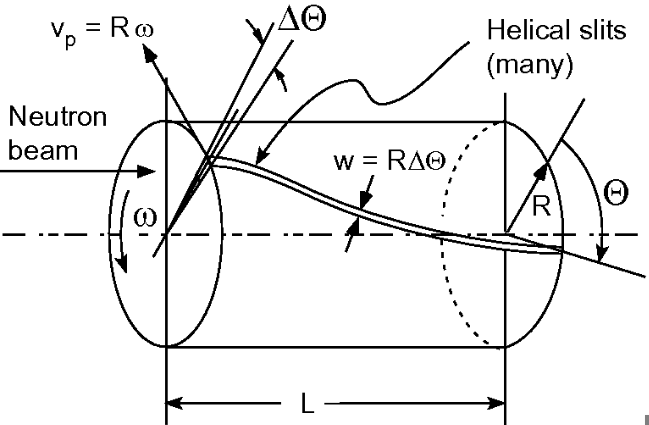
\includegraphics[width=0.45\textwidth]{neutron_v_selector.png}
  \caption{Elements of Slow-Neutron Scattering, \href{https://doi.org/10.1017/CBO9781139029315}{https://doi.org/10.1017/CBO9781139029315}}
\end{wrapfigure}

W celu uzyskania monochromatycznej wiązki neutronów stosuje się 
mechaniczne selektory prędkości. Selektor ma postać obracającego się 
cylindra o długości $L$ z helikalną szczeliną o kącie skrętu $\Theta$ i 
szerokości kątowej $\Delta\Theta$. Wiązka neutronów padających 
na selektor przechodzi wcześniej przez kolimator, który przepuszcza 
tylko neutrony poruszające się wzdłuż osi selektora.

Proszę obliczyć:
\begin{itemize}
    \item średnią prędkość $v_p$ neutronów  o temperaturze $T$,
    \item prędkość kątową selektora który przepuszcza neutrony o $v_p$
          przez środek szczeliny,
    \item zakres prędkości $[v_{\min}, v_{\max}]$ przepuszczanych przez szczelinę
          o szerokości $\Delta\Theta$.
    \item ułamek $r$ neutronów o temperaturze $T$ przepuszczanych przez selektor
          (całkę można wykonać numerycznie).
\end{itemize}
\vspace{1cm}
Parametry selektora i gazu: $T = 310\,\text{K}$, 
$L = 0.8\,\text{m}$, $\Theta = 0.25$, 
$\Delta\Theta = 0.02$. 
Masę neutronu i stałą Boltzmanna można znaleźć w tablicach.


\begin{solution}

Średnia prędkość $v_p$ neutronów o temperaturze $T$. Zakładamy że 
neutrony mają rozkład prędkości Maxwella-Boltzmanna tylko dla jednej osi 
(wzdłuż osi selektora):


\begin{align*}
  \langle v_x \rangle = \int_0^\infty v_x f(v_x) dv_x  = 
  \left( \frac{m}{2\pi k_B T} \right)^{1/2} 
  \int_0^\infty v_x \exp\left( -\frac{m v_x^2}{2 k_B T} \right) dv = \\
 \left( \frac{m}{2\pi k_B T} \right)^{1/2}  \frac{1}{2} \int_{0}^{\infty} \exp\left( -\frac{m v_x^2}{2 k_B T} \right) dv^{2}_x =\\
  \left( \frac{m}{2\pi k_B T} \right)^{1/2}  \frac{1}{2} \frac{2 k_B T}{m} = 
  \sqrt{\frac{k_B T}{2\pi m}} = 628\,\text{m/s} 
\end{align*}



Kąt skrętu $\Theta$ oznacza, że na jednostkę długości cylindra kanał odchyla się 
\begin{align*}
\delta \phi = \Theta / L
\end{align*} 

W czasie $dt$ neutron przebywa drogę $dz = v dt$ w głąb cylindra. 
Dla nieruchomego cylindra kanał będzie odchylony o kąt 
\begin{align*}
\delta \phi dz = \Theta v dt / L
\end{align*}

Cylinder musi się obrócić o ten sam kąt, aby kanał był skierowany na wylot. 
Oznacza to, że prędkość kątowa selektora musi spełniać warunek:
\begin{align*}
\omega dt = \Theta v dt / L \implies \omega = \frac{\Theta v}{L} 
= \frac{0.25 \cdot 628}{0.8} = 196\,\text{rad/s} = 31\,\text{Hz}
\end{align*}

Zakres prędkości przepuszczanych przez szczelinę o szerokości $\Delta\Theta$:
\begin{align*}
\Delta \phi = \Delta\Theta / L \implies \Delta v = \frac{\Delta\Theta v}{\Theta} = 
\frac{0.02 \cdot 628}{0.25} = 50\,\text{m/s}
\end{align*}

Ułamek neutronów o temperaturze $T$, trafiających w szczelinę
i przepuszczanych przez selektor:
\begin{align*}
r = \int_{v_p - \Delta v/2}^{v_p + \Delta v/2} f(v) dv = 
\left( \frac{m}{2\pi k_B T} \right)^{1/2} 
\int_{v_p - \Delta v/2}^{v_p + \Delta v/2} \exp\left( -\frac{m v^2}{2 k_B T} \right) dv \approx  
0.01
\end{align*}

Kod Python do numerycznej całki:
\begin{verbatim}
from scipy.stats import maxwell, norm
from scipy.constants import k as kB
from scipy.constants import proton_mass as m
import numpy as np
import matplotlib.pyplot as plt

T = 310 #K
delta_v = 50 #m/s

scale = np.sqrt(kB * T / m)
v_p = np.sqrt(kB * T / (2 * np.pi * m))
v_min = v_p - delta_v / 2
v_max = v_p + delta_v / 2

r = norm(loc=v_p, scale=scale).cdf(v_max) - norm(loc=v_p, scale=scale).cdf(v_min)
print("Velocity range: [{:3.2f}, {:3.2f}] m/s".format(v_min, v_max))
print("Ratio for 1D = {:3.2f}".format(r))
\end{verbatim}

\newpage
\end{solution}
%%%%%%%%%%%%%%%%%%%%%%%%%%%%%%%%%%%%%%%%%%%%%%%%%%%%%%
\zaddom[]

Reakcje termojądrowe w Słońcu zachodzą w temperaturze około 
$T = 1.5 \cdot 10^7\,\text{K}$. Proszę:
\begin{itemize}
  \item obliczyć średnią energię kinetyczną protonów Słońcu: $\langle E_k \rangle$.
  \item energię kinetyczną wymaganą by protony zbliżyły się do siebie na 
        odległość rzędu ich rozmiaru: $V_{0}$.
  \item oszacować ułamek protonów w Słońcu, które mają prędkość większą niż ta 
        z poprzedniego punktu: $r$.
\end{itemize}

Proszę przyjąć promień neutron  $r_{0} = 0.8 \cdot 10^{-15}\,\text{m}$.
Masa protonu: $m_p = 1.67 \cdot 10^{-27}\,\text{kg}$,
stała Boltzmanna: $k_B = 1.38 \cdot 10^{-23}\,\text{J/K}$.
Energię proszę wyrazić w keV (1 eV = $1.6 \cdot 10^{-19}\,\text{J}$).

\begin{solution}

Energia wymagana by neutrony zbliżyły się do siebie na odległość rzędu ich rozmiaru:
\begin{align*}
V_0 = \frac{1}{4\pi \epsilon_0} \frac{e^2}{r_{0}} = \frac{1}{4\pi \cdot 8.85 \cdot 10^{-12}} \cdot \frac{(1
.6 \cdot 10^{-19})^2}{0.8 \cdot 10^{-15}} = 2.3 \cdot 10^{-13}\,\text{J} = 1800\,\text{keV}
\end{align*}

Porównujemy tę energię z energią kinetyczną ruchu względnego protonów w Słońcu:
\begin{align*}
\langle E_k \rangle = \frac{1}{2} m \langle v^{2} \rangle
\end{align*}

Ruch względny uwzględniamy używając masy zredukowanej $\mu = m_p / 2$ w 
rozkładzie Maxwella-Boltzmanna:
\begin{align*}
\langle v^{2} \rangle = \frac{3}{2} \frac{2 k_B T}{\mu} = \frac{6 k_B T}{m}
\end{align*}

Stąd średnia energia kinetyczna ruchu względnego protonów w Słońcu
Używamy masy rzeczywistej, bo interesuje nas energia kinetyczna jednego protonu w układzie spoczynkowym drugiego,
a nie całkowita energia kinetyczna układu dwóch protonów.

\begin{align*}
\langle E_k \rangle = \frac{1}{2} m \langle v^{2} \rangle = 
\frac{1}{2} m \cdot \frac{6 k_B T}{m} = 3 k_B T = 
3 \cdot 1.38 \cdot 10^{-23} \cdot 1.5 \cdot 10^7 = 6.2 \cdot 10^{-16}\,\text{J} = 3.9\,\text{keV}
\end{align*}

Trzeba jednak pamiętać, że połowa par się oddala od siebie, a połowa zbliża.


Ułamek protonów w Słońcu, które mają wystarczającą energię do zbliżenia się 
na odległość rzędu rozmiaru neutronu:
\begin{align*}
r = \int_{v_0}^\infty f(\Delta v) d^{3} \Delta v = 
4\pi \left( \frac{\mu}{2\pi k_B T} \right)^{3/2} 
\int_{v_0}^\infty \Delta v^2 \exp\left( -\frac{\mu \Delta v^2}{2 k_B T} \right) dv
\end{align*} 

Całka:
\begin{align*}
  \int_{x_0}^\infty x^2 e^{-a x^2} dx = || u = x,~ dv = x e^{-a x^2} dx, ~ v = -\frac{1}{2a} e^{-a x^2} || = \\
  -\frac{x}{2a}\exp(-a x^2) + \frac{1}{2a} \int_{x_0}^\infty e^{-a x^2} dx 
\end{align*}

Oszacujmy wielkość argumentu wykładnika dla $V_0$:
\begin{align*}
k_B T = 1.38 \cdot 10^{-23} \cdot 1.5 \cdot 10^7 = 2.07 \cdot 10^{-16}\,\text{J} = 1.3\,\text{keV} \\
\frac{V_0}{2k_B T} = \frac{1800~\text{keV}}{2 \cdot 1.3~\text{keV}} \simeq 700 \to
\exp\left( -\frac{V_0}{2k_B T} \right) \simeq 10^{-304}
\end{align*}

Całkę można więc oszacować zachowując jedynie pierwszy wyraz:
\begin{align*}
\int_{\Delta v_0}^\infty \Delta v^2 \exp\left( -\frac{\mu \Delta v^2}{2 k_B T} \right) d\Delta v \simeq
\frac{\Delta v}{2}\frac{2k_B T}{\mu} \exp\left( -\frac{\mu \Delta v^2}{2 k_B T} \right) \Bigg|_{\Delta v_0}^\infty =
\frac{\Delta v_0}{2}\frac{k_B T}{\mu} \exp\left( -\frac{\mu \Delta v_0^2}{k_B T} \right)
\end{align*}

Ostatecznie, uwzględniając, że tylko połowa par protonów zbliża się do siebie, otrzymujemy:
\begin{align*}
f = \simeq 0.5 \cdot 4\pi \left( \frac{\mu}{2\pi k_B T} \right)^{3/2} \cdot \frac{\Delta v_0}{2}\frac{2k_B T}{\mu} \exp\left( -\frac{\mu \Delta v_0^2}{2 k_B T} \right) = \\
\frac{2\pi}{(2\pi)^{3/2}}\left( \frac{\mu}{2\pi k_B T} \right)^{1/2} \frac{\Delta v_0}{2} \exp\left( -\frac{V_0}{2k_B T} \right) 
\end{align*}

Więc ułamek protonów w Słońcu, które mają wystarczającą energię do zbliżenia się na odległość 
rzędu rozmiaru neutronu jest rzędu $10^{-304}$...

\newpage
\end{solution}

%%%%%%%%%%%%%%%%%%%%%%%%%%%%%%%%%%%%%%%%%%%%%%%%%%%%%%%%
\zaddom[]

Korzystając z rozkładu Maxwella-Boltzmanna proszę znaleźć rozkład
prawdopodobieństwa dla energii kinetycznej.

\begin{solution}

Rozkład prędkości Maxwella-Boltzmanna w funkcji prędkości $v$ jest dany wzorem:
\begin{align*}
f(v) = 4\pi \left( \frac{m}{2\pi k_B T} \right)^{3/2} v^2 \exp\left( -\frac{m v^2}{2 k_B T} \right)
\end{align*}
  
Rozkład w funkcji energii otrzymujemy całkując rozkład prędkości z warunkiem $E = \frac{1}{2} m v^2$:
\begin{align*}
f(E) = \int_0^\infty f(v) \delta\left(E - \frac{1}{2} m v^2\right) dv = 
\int_0^\infty f(v) \frac{\delta(v - \sqrt{2E/m})}{\sqrt{2 m E}} dv = \\
= 4\pi \left( \frac{m}{2\pi k_B T} \right)^{3/2} \cdot \frac{2E}{m} \exp\left( -\frac{E}{k_B T} \right) \cdot \frac{1}{\sqrt{2 m E}} = 
2 \sqrt{\frac{E}{\pi}} \left( \frac{1}{k_B T} \right)^{3/2} \exp\left( -\frac{E}{k_B T} \right)
\end{align*}


\newpage  
\end{solution}
%%%%%%%%%%%%%%%%%%%%%%%%%%%%%%%%%%%%%%%%%%%%%%%%%%%%%%%%
\end{document}